%% -*- coding:utf-8 -*-
\chapter{Clause types and expletives}
\label{chap-expletives}

Yiddish besseres Beispiel nehmen, das wirklich V2 zeigt.

\if0


\subsection{Eingebettete Sätze}

\subsubsection{Sätze mit Komplementierer}

\frame{
\frametitle{Deutsch: Komplementierer + Verbletzt, ohne Inversion}

\vfill
\centerfit{\begin{tikzpicture}
\tikzset{level 1+/.style={level distance=2\baselineskip}}
\tikzset{frontier/.style={distance from root=9\baselineskip}}
\Tree[.CP
       [.C dass ]
       [.S
        [.{NP[\type{nom}]} niemand ]
        [.V$'$
          [.{NP[\type{acc}]} ihn ]
          [.V kennt ]
           ] ] ]
\end{tikzpicture}}


}


\frame{
\frametitle{Englisch: Komplementierer + SVO}


\vfill


\centerfit{\begin{tikzpicture}
\tikzset{level 1+/.style={level distance=2\baselineskip}}
\tikzset{frontier/.style={distance from root=9\baselineskip}}
\Tree[.CP
       [.C that ]
       [.S
        [.{NP[\type{nom}]} nobody ]
        [.VP
          [.V  knows ]
          [.{NP[\type{acc}]} him ] ] ] ]
\end{tikzpicture}}





}


\frame{
\frametitle{Jiddisch: Komplementierer + V2}



\centerfit{\scalebox{.6}{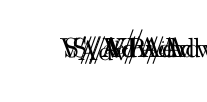
\begin{tikzpicture}[
level 1+/.style={level distance=2\baselineskip},
frontier/.style={distance from root=16\baselineskip},
connect/.style={semithick,<->,color=green}]
\tikzset{every tree node/.style={align=center,anchor=north}}
%\draw (-3,-5) to[grid with coordinates] (4,0);
\Tree[.CP
        [.C az\\dass ]
        [.S
          [.\node (Adv) {Adv}; haynt$_i$\\heute ]
          [.\node (S/Adv) {S/Adv};
            [.{V \sliste{ S/\!/V }} 
              [.V hot$_k$\\hat ] ]
            [.\node (S//V/Adv) {S$/\!/$V/Adv};
              [.NP Max\\Max ]
              [.\node (V/V/Adv) {V$'\!/\!/$V/Adv};
                [.{V$\!/\!/$V}  \_$_k$ ]
                [.\node (VP/Adv) {VP/Adv}; 
                  [.VP
                    [.V geleyent\\gelesen ]
                    [.NP \edge[roof]; {dos bukh}\\{das Buch} ] ]
                  [.\node (Adv/Adv) {Adv/Adv}; \_$_i$ ] ] ] ] ] ] ]
%% \draw[connect] (Adv/Adv.north east)   [bend right] to (VP/Adv.south east);
%% \draw[connect] (VP/Adv.north east)    [bend right] to (V/V/Adv.south east);
%% \draw[connect] (V/V/Adv.north east)   [bend right] to (S//V/Adv.south east);
%% \draw[connect] (S//V/Adv.north east)  [bend right] to (S/Adv.east);
%% \draw[connect] (S/Adv.north east)     [bend right] to (Adv);
\end{tikzpicture}}}



\ea
\gll Ikh meyn  az   haynt hot Max geleyent dos bukh.\footnotemark\\
     ich   denke dass heute hat Max gelesen   das Buch\\
\footnotetext{\citew[\page 58]{Diesing90a}.}
\glt `Ich denke, dass Max heute das Buch gelesen hat.'
\z

}


\subsubsection{Positionionale Expletiva}

\frame{
\frametitle{Positionale Expletiva}

\begin{itemize}
\item Deutsch, Dänisch, Jiddish, \ldots erlauben Expletiva vor dem finiten Verb:

\ea[]{
Es ritten drei Reiter zum Tor hinaus.
}
\z



\end{itemize}

}


\subsubsection{Interrogativnebensätze}

\frame{
\frametitle{Deutsch: \emph{w} + SOV}

\vfill

\centerfit{\begin{tikzpicture}[
level 1+/.style={level distance=2\baselineskip},
frontier/.style={distance from root=10\baselineskip},
connect/.style={semithick,<->,color=green}]
\tikzset{every tree node/.style={align=center,anchor=north}}
%\draw (-3,-5) to[grid with coordinates] (4,0);
\Tree[.S
       [.{NP[\snom]} wer ]
       [.S/NP 
         [.NP/NP \trace{} ]
         [.V$'$
           [.{NP[\sacc]} \edge[roof]; {das Buch} ]
           [.V liest ] ] ] ]
\end{tikzpicture}}

}

\frame{
\frametitle{Danish: \emph{w}-Subjekt + Expl + VO}

\vfill

\centerfit{\scalebox{0.9}{\begin{tikzpicture}[
level 1+/.style={level distance=3\baselineskip},
frontier/.style={distance from root=15\baselineskip},
connect/.style={semithick,<->,color=green}]
\tikzset{every tree node/.style={align=center,anchor=north}}
%\draw (-3,-5) to[grid with coordinates] (4,0);
\Tree[.S
       [.{NP[\snom]} hvem\\wer ]
       [.{S/NP[\snom]}
         [.{NP[\lnom]} det\\{\sc expl} ]
         [.{VP/NP[\snom]}
           [.{V$'$/NP[\snom]}
             [.V læser\\liest ]
             [.{NP[\snom]/NP[\snom]} \trace{} ] ]
           [.{NP[\sacc]} bogen\\Buch.{\sc def} ] ] ] ]
\end{tikzpicture}}}



}


\frame{
\frametitle{Jiddish: \emph{w}-Subjekt + V2 mit Expletivum im VF}





\vfill

\centerfit{\scalebox{0.65}{\begin{tikzpicture}[
level 1+/.style={level distance=3\baselineskip},
frontier/.style={distance from root=21\baselineskip},
connect/.style={semithick,<->,color=green}]
\tikzset{every tree node/.style={align=center,anchor=north}}
%\draw (-3,-5) to[grid with coordinates] (4,0);
\Tree[.S
       [.{NP[\snom]} ver$_i$\\wer ]
       [.{S/NP[\snom]}
         [.{NP[\lnom]} es$_j$\\{\sc expl} ]
         [.{S/NP[\snom]/NP[\lnom]}
           [.{V \sliste{S//V}}
             [.V leyent$_k$\\liest ] ]
           [.{S//V/NP[\snom]/NP[\lnom]}
             [.{NP[\lnom]/NP[\lnom]} \trace$_j$ ] 
             [.{VP//V/NP[\snom]}
               [.{V$'$//V} 
                 [.V//V \trace$_k$ ]
                 [.{NP[\snom]/NP[\snom]} \trace$_i$ ] ]
               [.{NP[\sacc]} bogen\\Buch.{\sc def} ] ] ] ] ] ]
\end{tikzpicture}}}


}


\frame{
\frametitle{Expletiva im Deutschen und Jiddischen}


\begin{itemize}
\item Diese können nicht im Mittelfeld stehen:
\eal
\ex[]{
Es arbeiten noch drei Männer.
}
\ex[*]{
dass es noch drei Männer arbeiten
}
\zl
\pause
\item Beschränkung, die verlangt, dass diese Elemente extrahiert sein müssen.

\pause
\item Aber:
\ea[*]{
Es$_i$ glaube ich, dass \_$_i$ noch drei Männer arbeiten.
}
\z
\pause
\item Voranstellung von Expletivpronomina über Satzgrenzen muss ohnehin ausgeschlossen werden:
\ea[*]{
Es$_i$ glaube ich, dass \_$_i$ regnet.
}
\z


\end{itemize}






}
\fi
